%%%%%%%%%%%%%%%%%%%%%%%%%%%%%%%%%%%%%%%%%
% Dictionary
% LaTeX Template
% Version 1.0 (20/12/14)
%
% This template has been downloaded from:
% http://www.LaTeXTemplates.com
%
% Original author:
% Vel (vel@latextemplates.com) inspired by a template by Marc Lavaud
%
% License:
% CC BY-NC-SA 3.0 (http://creativecommons.org/licenses/by-nc-sa/3.0/)
%
%%%%%%%%%%%%%%%%%%%%%%%%%%%%%%%%%%%%%%%%%

%----------------------------------------------------------------------------------------
%	PACKAGES AND OTHER DOCUMENT CONFIGURATIONS
%----------------------------------------------------------------------------------------

\documentclass[10pt,a4paper,twoside]{article} % 10pt font size, A4 paper and two-sided margins

\usepackage[top=3.5cm,bottom=3.5cm,left=3.7cm,right=4.7cm,columnsep=30pt]{geometry} % Document margins and spacings

\usepackage[utf8]{inputenc} % Required for inputting international characters

\usepackage[T1]{fontenc} % Output font encoding for international characters

\usepackage{polyglossia}
\setdefaultlanguage{english}
\setotherlanguages{russian,ukrainian,chinese,turkish,arabic,french,italian,spanish}
\setmainfont{Helvetica} % font book but only system fonts
\newfontfamily\cyrillicfont[Script=Cyrillic]{Helvetica}


\usepackage{fontspec}

% \usepackage[T2A]{fontenc}      % Font encoding for Cyrillic
% \usepackage[utf8]{inputenc}     % Input encoding for UTF-8
% \usepackage[ukrainian]{babel}   % Ukrainian language support

\usepackage{times} % Use the Palatino font

\usepackage{microtype} % Improves spacings

\usepackage{multicol} % Required for splitting text into multiple columns

\usepackage[bf,sf,center]{titlesec} % Required for modifying section titles - bold, sans-serif, centered

\usepackage{fancyhdr} % Required for modifying headers and footers
\fancyhead[L]{\textsf{\rightmark}} % Top left header
\fancyhead[R]{\textsf{\leftmark}} % Top right header
\renewcommand{\headrulewidth}{1.4pt} % Rule under the header
\fancyfoot[C]{\textbf{\textsf{\thepage}}} % Bottom center footer
\renewcommand{\footrulewidth}{1.4pt} % Rule under the footer
\pagestyle{fancy} % Use the custom headers and footers throughout the document

\newcommand{\entry}[4]{\markboth{#1}{#1}\textbf{#1}\ {(#2)}\ \textit{#3}\ $\bullet$\ {#4}}  % Defines the command to print each word on the page, \markboth{}{} prints the first word on the page in the top left header and the last word in the top right

\usepackage{tikz}
\usetikzlibrary{calc} % Optional, but useful for more complex calculations




%----------------------------------------------------------------------------------------

\begin{document}

%----------------------------------------------------------------------------------------
%	TITLE PAGE
%----------------------------------------------------------------------------------------


\begin{titlepage}

\AddToHookNext{shipout/background}{
    \begin{tikzpicture}[remember picture, overlay]
        \node at ($(current page.south) + (0, 8.25cm)$) % Adjust 1cm for desired distance from bottom
            {\centering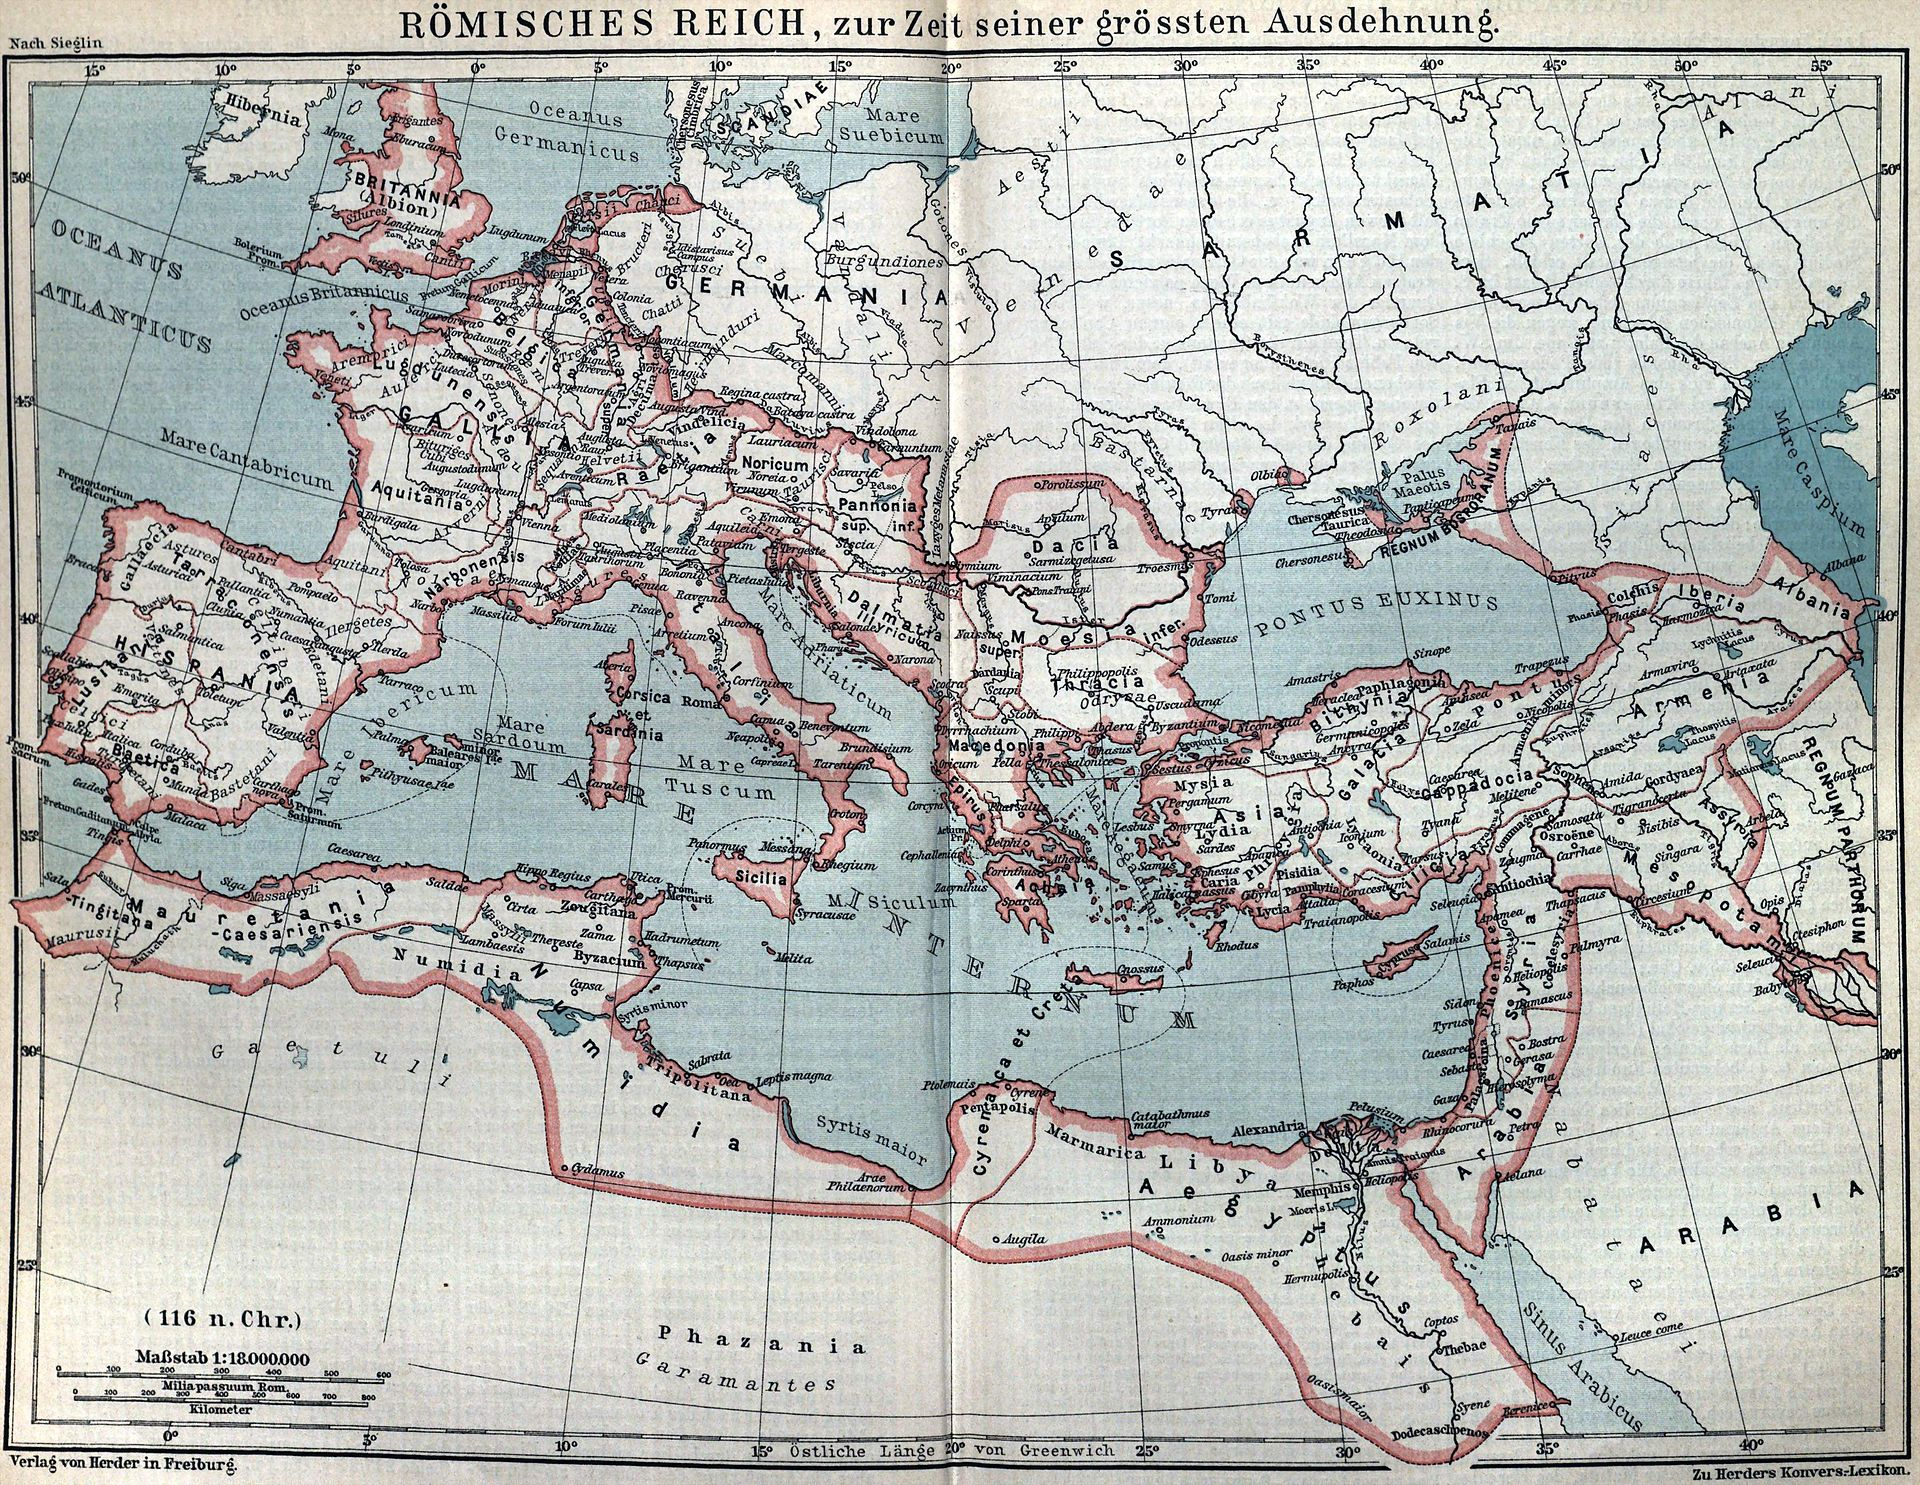
\includegraphics[width=1.5\textwidth]{Regnum_Bosporanum}}; % Adjust width and image filename
    \end{tikzpicture}
}


  \centering % Center all content
    \vspace*{2cm} % Add vertical space from the top
    {\Huge Xersonesus \\} % Large title
    \vspace{1cm}
    {\Large An Historical and Critical Encyclopedia of the Ukraine War \\} % Subtitle
    \vspace{2cm}
    {\Large 3AC3B33B33B53BB3BF3C2 \\} % Author name
    {\normalsize \emph{ seppie coi piselli alla romana } \\}
    \vspace{1cm}
    {\today} % Date
    \vfill % Fill remaining vertical space
    % Add any other elements like logos, disclaimers, etc.


 \end{titlepage}

%----------------------------------------------------------------------------------------
%	SECTION A
%----------------------------------------------------------------------------------------

\section*{A}

\begin{multicols}{2}

\entry{Artemovsk} {Artemovsk} {Noun} {See \textbf{Bakhmut-Artemovsk}.}

\entry{Artillery} {ar·til·ler·y} {Noun} {Coined by the gravedigger of the revolution, Joseph Stalin, artillery is the god of war. The god of war, however, is now but only a vital component in an evolving array of combined arms in eastern Europe. In the beginning of the Ukraine war the  media focused almost exclusively on parity. The number of Russian artillery guns, calibre, the number of munitions, the type of munitions, or the way in which the Russians accurately targeted Ukrainian targets demonstrated the advantage Russia weaned over its opponent.  \newline \indent In the beginning of the Ukraine war, primarily before the great Ukrainian offensive in Kharkiv, launched on September 6th, 2022 but prepared weeks in advance, until the end of Ukraine's 'Spring' counteroffensive in 2023, artillery played a dominant role on the battlefield. Ukraine's failed 'Spring' counteroffensive witnessed confirmed Russia's seizure of the strategic initiative after the fall of Bakhmut-Artemovsk on May 23rd, 2023. In the winter of 2023 the Ukraine war witnessed a major transformation in the deployment of drones. Ukraine began to mass produce First Person View drones to strengthen its defense of the Donbas in the face of continued Russian advances. Necessity is the mother of invention. Ukraine's FPV drones began to play a dominant role on the battlefield, overtaking but by no means substituting for the role artillery played in the beginning of the war. The first Ukrainian brigades with dedicated, trained, expert drone pilots began to take shape. }



\end{multicols}

%----------------------------------------------------------------------------------------
%	SECTION B
%----------------------------------------------------------------------------------------

\section*{B}

\begin{multicols}{2}

\entry{Bakhmut-Artemovsk} {} {} {The city whose fall sounded a death knell for the Ukrainian strategic initiative. Spellt \textukrainian{Бахмут — Артемівськ} in Ukrainian but —  \textrussian{Бахмут — Артемовск} in Russian, the city's history is unique.  }

\entry{Bombing} {bomb·ing} {Gerund} {Bombing has thus far been ineffective from the beginning of the Ukraine war. It alone has not accomplished a single strategic objective for any of the warring parties. \newline \indent The \emph{New York Times} is one of the most fervent advocates of bombing.\footnote{“How to Choke Iraq,” \emph{NYT}, December 7th, 1990.} \footnote{“Bombing Iraq Ins’t Enough,” \emph{NYT}, January 30th, 1998.} \footnote{“American Bombs Make Iraq Stronger,” \emph{NYT}, December 20th, 1998.} \footnote{“Bomb North Korea, Before It’s Too Late,” \emph{NYT}, April 12th, 2013.} \footnote{“Bomb Syria, Even if It is Illegal,” \emph{NYT}, August 27th, 2013. } \footnote{“To Stop Iran’s Bomb, Bomb Iran,” \emph{NYT}, March 26th, 2015.}

}

\end{multicols}


%----------------------------------------------------------------------------------------
%	SECTION C
%----------------------------------------------------------------------------------------

\section*{C}

\begin{multicols}{2}

\entry{CIA} {Abbreviation} {Noun} {

It is often claimed in print that the CIA (Central Intelligence Agency) predicted the beginning of the Ukraine war. It is true. The CIA forecast Russia's full-scale invasion less than two weeks in advance. \footnote{ It is hard to imagine a time before the \emph{Kyiv Independent}, the newspaper the \emph{Wall Street Journal} tapped to cover the Ukraine war with the immediacy the U.S.-led NATO alliance demands for its rolling propaganda. \textukrainian{\emph{Українська правда}}, however, is one of the few Ukrainian newspapers whose history of publication precedes the struggle for Ukraine. It is thus a newspaper preceding the \emph{Kyiv Independent}'s coverage on the Ukraine war. It published the majority of the articles covering the CIA's predictions. In one of these articles, the headline describes the attack to be within days: \textukrainian{"Байден вважає, що Путін може напасти на Україну в найближчі дні} – The Guardian," \textukrainian{\emph{Українська правда}}, 11 \textukrainian{лютого} 2022. The first of these is reporting on \emph{The Guardian}. It is a reference to the \emph{The Guardian}'s article published on February 11th under the title, "US warns of ‘distinct possibility’ Russia will invade Ukraine within days." Reporting on \emph{Der Spiegel} revealed the date: ["\textukrainian{ЦРУ назвало імовірну дату нападу Росії на Україну} – \emph{Spiegel}," \textukrainian{\emph{Українська правда}}, 11 \textukrainian{Лютого} 2022]. A reference to the \emph{Der Spiegel}'s article published on February 11th under the title, "CIA rechnet mit russischem Angriff kommende Woche," the so-called \textukrainian{імовірна дата} could not have been vague in German. Another published a day after these read: ["\textukrainian{Головні новини п’ятниці та ночі: ймовірний напад Росії, санкції РНБО}, \textukrainian{\emph{Українська правда}}, 12 \textukrainian{Лютого} 2022"].} In the publications in Ukrainian, Hebrew, Russian, or English, the majority of the accompanying images are pulled directly from an article published seven years ahead of its time. On Mar 9, 2015, \emph{Stratfor} published its famous article, "Gaming a Russian Offensive." The scenarios the CIA discusses in its forecast are replications of those from \emph{Stratfor}'s article. The arrows in these sets of images follow those in \emph{Stratfor}'s article.  \newline \indent It is interesting how these new images spiral outward from a common source almost like a Fibonacci sequence, adding more arrows with the fractionalization of the original scenarios.  In one of the articles published by \textukrainian{\emph{Українська правда}}, the newspaper reports on February 12th how \textukrainian{"Росія має 9 маршрутів сэргнення до України, танки можуть сягнути Києва за 2 доби - розвідка США"}. A few of these nine routes, as impractical as the aforementioned fractionalization, could not have been farther from the truth, as the Russia massed scores of Russian troops on the highways into the Donbas, where the majority of the fighting raged for years before Russia launched its full-scale invasion. These three additional scenarios exceed \emph{Stratfor's} original six. 

}


\end{multicols}


%----------------------------------------------------------------------------------------
%	SECTION D
%----------------------------------------------------------------------------------------

\section*{D}

\begin{multicols}{2}

\entry{Delta} {Title} {Software} {Seldom mentioned in the media, Delta is a battlefield management system preceding the U.S. Army's phased released of its own Large Language Models for AI. Announced by Col. Jonathan Harvey from the U.S. Army on October 18th, 2025, the "sufficient, joint weapon target pairing Large Language Model (LLM)" is scheduled to run inside of the "kill chain," a model advancing from a simple exercise to a "fully devolved reasoning model." The most likely set of data is based on multiple projects running simultaneously in the field of artillery. One of these relates to completing the updates to NATO's firing tables, military artillery data sheets used for calculating trajectories, for the first time since the Cold War.\footnote{["NATO to make fresh push for common arms standards," \emph{Reuters} October 16th, 2024} Another is likely the collocation of manuals on targeting, tactics, techniques or procedures\footnote{[https://www.cia.gov/readingroom/docs/CIA-RDP07S00452R000300820008-6.pdf]} for field artillery in combination with the aforementioned firing tables. In the face of the revolution the U.S. Army's phased release of its own Large Language Models is expected to achieve for combat manage systems like Delta, Delta is legacy. 

In the first year of the Ukraine war, a Russian affiliated hacker managed to gain access to a Ukrainian commander's laptop with Delta. 

}


\entry{The Department of Defense} {Title} {Phrase} {In recognition of the role warfare plays in policy, the Trump administration reversed years of intellectually debased stagnation in the U.S. Armed Forces' bureaucracy with the elimination of the Department of Defense for the return of the Department of War during the Ukraine war. 

}


\end{multicols}

%----------------------------------------------------------------------------------------
%	SECTION R
%----------------------------------------------------------------------------------------

\section*{R}

\begin{multicols}{2}

\entry{Russia} {Russ·ia} {Noun} {

Russia is one of the belligerents in the Ukraine war. In comparison to Ukraine, Russia's history of war in the area from the Black to the Baltic seas is extensive. 


}
\end{multicols}



%----------------------------------------------------------------------------------------
%	SECTION S
%----------------------------------------------------------------------------------------

\section*{S}

\begin{multicols}{2}

\entry{Sanctions} {Sanct·ions} {Noun} {

The collapse of Syria's Assad regime, a fifty year old dynasty, is a result of the Ukraine war. 

}


\entry{Shahed} {Sha·hed} {Noun} {

Russia launched its first Shahed, one of the most important evolving weapons in the Ukraine war, in the immediate aftermath of its defeat in the face of the great Ukrainian offensive in Kharkiv   launched on September 6th, 2022. \newline \indent Debate rages around the modifications, versions, or models of Shaheds involved in legendary attacks, which Russian or Iranian factory produced them, the country of origin responsible for, or the actual nature, underlying engineering, or specification of the most distinguished parts, components or kits.  

}

\entry{Syria} {Syr·ia} {Noun} {
The collapse of Syria's Assad regime, a fifty year old dynasty, is a result of the Ukraine war. 

}


\end{multicols}


%----------------------------------------------------------------------------------------
%	SECTION T
%----------------------------------------------------------------------------------------

\section*{T}

\begin{multicols}{2}

\entry{Time} {Ti·me} {Noun} {

It is to be determined which of the most prized possessions in warfare, time or space, the belligerents seek or exploit at any given phase of the Ukraine war. 

}


\end{multicols}

%------------------------------------------------
\end{document}